\chapter{AI trong n8n - Xu hướng và ứng dụng}
Chào mừng bạn đến với một trong những phần thú vị nhất của n8n: tích hợp trí tuệ nhân tạo! Nếu bạn nghĩ rằng tự động hóa quy trình công việc đã tuyệt vời rồi, thì việc thêm AI vào n8n sẽ đưa mọi thứ lên một tầm cao mới.


\section{Giới thiệu về Large Language Model}
Mô hình ngôn ngữ lớn (Large Language Model - LLM) là mô hình học sâu được huấn luyện trên một lượng lớn dữ liệu ngôn ngữ tự nhiên mô phỏng hệ thần kinh con người vô cùng phức tạp để hiểu và tạo ra văn bản tự nhiên. LLM được phát triển dựa trên các kỹ thuật học sâu và sử dụng mạng nơ-ron tích chập, thường có hàng tỷ hoặc thậm chí hàng nghìn tỷ tham số để xử lý ngôn ngữ ở quy mô lớn. Các mô hình này có khả năng học hỏi từ lượng dữ liệu ngôn ngữ khổng lồ, giúp chúng có thể hiểu và tạo ra văn bản phức tạp, cũng như thực hiện các tác vụ ngôn ngữ khác nhau. 




\textbf{Đặc điểm của LLM}
\begin{itemize}
    \item Số lượng tham số lớn: Mô hình ngôn ngữ lớn chứa nhiều tham số, giúp lưu trữ thông tin và các mẫu ngôn ngữ phức tạp từ dữ liệu huấn luyện.

    \item Dự đoán từ tiếp theo: LLM sử dụng các thuật toán dự đoán từ tiếp theo để tạo ra văn bản dài và logic.

    \item Huấn luyện từ dữ liệu lớn: Được huấn luyện trên khối lượng dữ liệu văn bản khổng lồ từ nhiều nguồn, giúp mô hình hiểu đa dạng ngữ cảnh, phong cách, và ngữ pháp.

    \item Khả năng tổng quát: LLM có thể thực hiện nhiều tác vụ ngôn ngữ như dịch thuật, tóm tắt, trả lời câu hỏi và sáng tác văn bản. 
\end{itemize}


Kiến trúc của LLM chủ yếu bao gồm nhiều lớp mạng nơ-ron, như recurrent layers, feedforward layers, embedding layers, attention layers. Các lớp này hoạt động cùng nhau để xử lý văn bản đầu vào và tạo dự đoán đầu ra.
\begin{itemize}
    \item Embedding layer chuyển đổi từng từ trong văn bản đầu vào thành biểu diễn vectơ nhiều chiều (high-dimensional). Những vec-tơ này nắm bắt thông tin ngữ nghĩa và cú pháp của từng đơn vị cấu tạo nên câu (từ hoặc token) và giúp mô hình hiểu được ngữ cảnh của văn bản.
    \item Feedforward layers gồm nhiều lớp được kết nối đầy đủ áp dụng các phép biến đổi phi tuyến tính cho các embedding vector đầu vào. Các lớp này giúp mô hình học các thông tin trừu tượng hơn từ văn bản đầu vào.
    \item Recurrent layers của LLM được thiết kế để diễn giải thông tin từ văn bản đầu vào theo trình tự. Các lớp này duy trì trạng thái ẩn được cập nhật ở mỗi bước thời gian, cho phép mô hình nắm bắt được sự phụ thuộc giữa các từ trong câu.
    \item Attention layers là một phần quan trọng khác của LLM, cho phép mô hình tập trung có chọn lọc vào các phần khác nhau của văn bản đầu vào. Cơ chế này giúp mô hình chú ý đến các phần có liên quan nhất của văn bản đầu vào và tạo ra các dự đoán chính xác hơn.
    \item Hầu hết các mô hình học sâu, học máy đều sựa trên Vectorizetion. Hàm softmax tạo ra các bộ trọng số để giúp mô hình nhớ lại bộ trong số nào là quan trọng.
\end{itemize}

Mô hình ngôn ngữ lớn hoạt động bằng cách dựa trên đoán từ tiếp theo (next predict token) dựa trên chuỗi từ trước đó đã được cung cấp. Nhiệm vụ này là bài toán \text{dự đoán xác suất có điều kiện}, trong đó mô hình tính toán xác suất của từ tiếp theo $t_{n+1}$ dựa trên toàn bộ ngữ cảnh trước đó $t_1, t_2, \ldots, t_n$.
    \[P(t_{n+1} | t_1, t_2, \ldots, t_n)\]
Trong đó:
\begin{itemize}
    \item $t_1, t_2, \ldots, t_n$: Là các token đã được cung cấp (chuỗi truy vấn, hay ngữ cảnh).
    \item $t_{n+1}$: Là token tiếp theo mà mô hình cần dự đoán.
    \item $P(t_{n+1} | t_1, t_2, \ldots, t_n)$: Là xác suất có điều kiện cho từ tiếp theo $t_{n+1}$ xuất hiện dựa trên các từ đã biết.
\end{itemize}


Token là một bộ mapping, tokenize là một cách chuyển không gian số sang dạng vector. Có nhiều cách tokenize:
\begin{itemize}
    \item Token theo từ điển, mỗi từ sẽ được chuẩn hóa dưới dạng số 1, 2, 3, 4,... Nhược điểm khi số lượng từ tăng và có một từ không ở trong từ điển thì bộ tokenize sẽ không dùng được nữa.
    \item tokenize theo các âm tiết (cách làm hiện tại của chatGPT.
\end{itemize}

Do tính chất sinh từng token một để tạo thành một câu trả lời hoàn chỉnh, các token sinh ra là xác xuất để xuất hiện câu trả lời dựa trên câu prompt mà người dùng nhập vào. Số lượng token sinh ra rất nhanh nên ta có thể tận dụng điều này để stream token hiển thị liên tiếp các từ để tăng trải nghiệm người dùng thay vì phải đợi LLM trả ra cả một câu rồi mới gửi kết quả cho người dùng.


\textbf{AI Là Gì Và Tại Sao Nó Quan Trọng Với n8n?}


AI, hay Trí tuệ nhân tạo, là khả năng của máy tính để thực hiện các nhiệm vụ thường đòi hỏi trí thông minh của con người. Trong bối cảnh tự động hóa công việc với n8n, AI có thể giúp:
\begin{itemize}
    \item Phân tích dữ liệu lớn và phức tạp
    \item Tự động hóa các quyết định dựa trên dữ liệu
    \item Xử lý ngôn ngữ tự nhiên (NLP) để hiểu và tạo văn bản
    \item Phân tích hình ảnh và video
    \item Dự đoán xu hướng và kết quả
\end{itemize}

Khi tích hợp AI vào quy trình làm việc n8n, bạn có thể tự động hóa các tác vụ phức tạp hơn và đưa ra quyết định thông minh hơn trong quy trình của mình.

Ví dụ nhé: Bạn muốn n8n tự động phân loại email khách hàng thành "tích cực" hay "tiêu cực"? AI có thể đọc nội dung email và làm điều đó. Hay bạn cần tạo một bài đăng mạng xã hội nhanh chóng? AI cũng có thể giúp viết nội dung dựa trên vài từ khóa bạn cung cấp. Khi kết hợp với n8n, AI trở thành "bộ não" giúp quy trình của bạn không chỉ nhanh mà còn thông minh.

n8n linh hoạt, cho phép bạn kết nối với các dịch vụ AI bên ngoài thông qua các node – những khối lệnh nhỏ trong quy trình làm việc của bạn. Các dịch vụ AI phổ biến mà bạn có thể tích hợp bao gồm:
\begin{itemize}
    \item OpenAI: Tạo văn bản, trả lời câu hỏi, hoặc phân tích dữ liệu.
    \item Google AI: Dịch thuật, nhận diện hình ảnh, hoặc xử lý ngôn ngữ tự nhiên.
    \item Hugging Face: Dùng cho các tác vụ như phân loại cảm xúc hoặc tạo nội dung.
\end{itemize}


\section{Các node AI trong N8N}
n8n không chỉ là một công cụ tự động hóa thông thường – nó còn là một nền tảng mạnh mẽ để tích hợp trí tuệ nhân tạo vào các quy trình của bạn. Trong chương này, chúng ta sẽ khám phá các node AI được tích hợp sẵn trong n8n, từ những công cụ đơn giản như phân tích cảm xúc đến các ứng dụng phức tạp hơn như trích xuất thông tin hay trả lời câu hỏi dựa trên dữ liệu. Qua đây ta hãy cùng tim fhieeur về chúng. 


\subsection{AI Agent}

\begin{figure}[htbp]
    \centering
    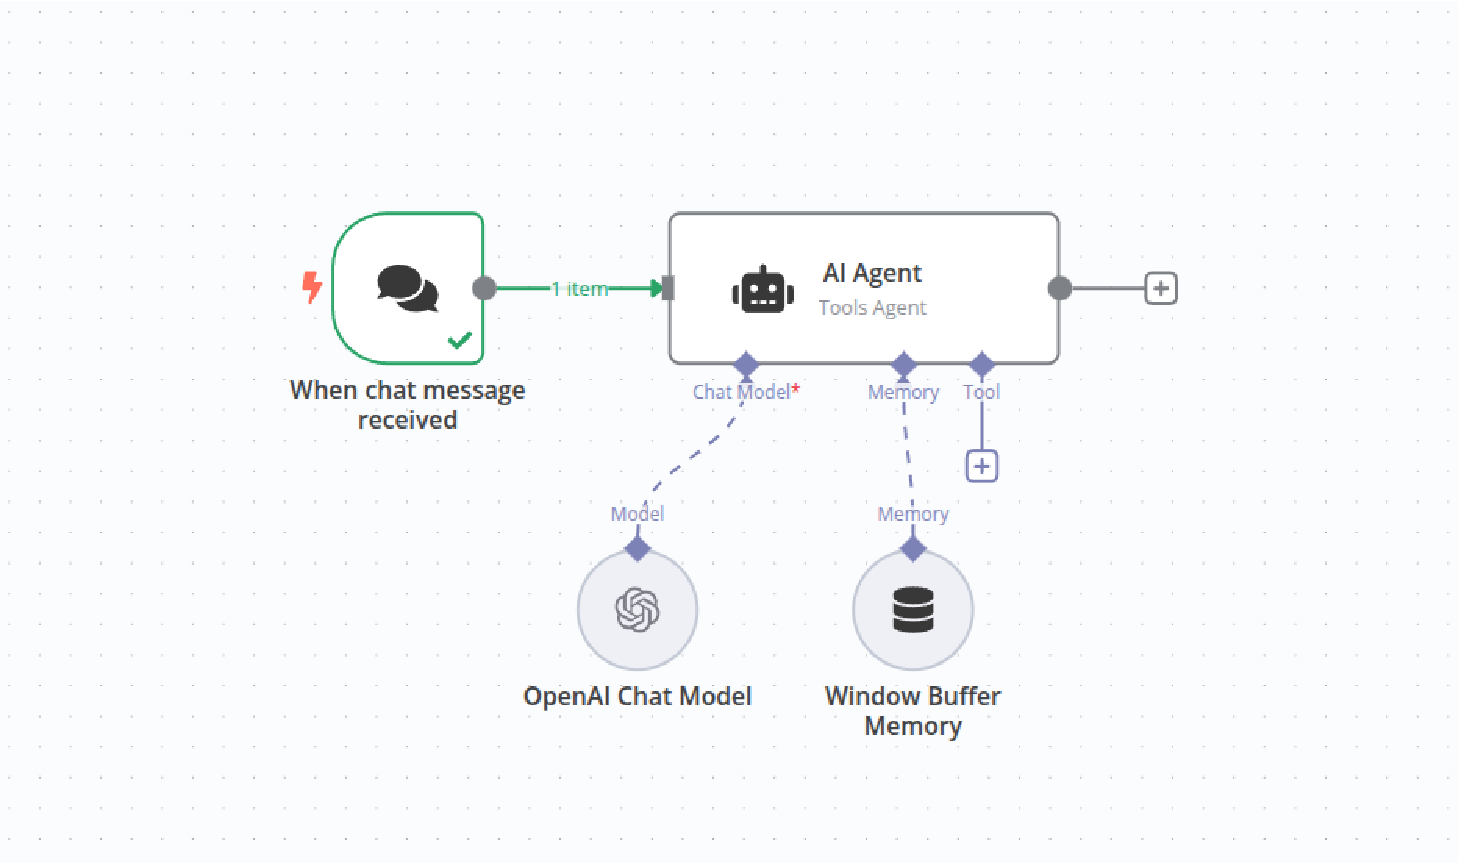
\includegraphics[width=1\linewidth]{Chap1-7/ai-intro01.pdf}
\end{figure}

AI Agent trong n8n là một node linh hoạt, đóng vai trò như một “trợ lý thông minh” trong các quy trình tự động hóa của bạn. Hãy tưởng tượng nó như một người bạn đồng hành có khả năng xử lý các tác vụ phức tạp mà không cần bạn phải viết mã từ đầu. AI Agent có thể được sử dụng để thực hiện nhiều nhiệm vụ khác nhau, từ trả lời câu hỏi, tạo nội dung, đến phân tích dữ liệu – tất cả đều dựa trên các mô hình ngôn ngữ lớn (LLM) mà bạn kết nối với nó.

Ví dụ, bạn có thể thiết lập một workflow để AI Agent tự động trả lời email khách hàng dựa trên nội dung họ gửi, hoặc phân loại các yêu cầu hỗ trợ trước khi chuyển đến đúng bộ phận. Để bắt đầu, bạn chỉ cần kết nối node này với một dịch vụ AI (như OpenAI) và định nghĩa nhiệm vụ cụ thể mà bạn muốn nó thực hiện. Đừng lo nếu bạn chưa quen – chúng ta sẽ đi qua từng bước thiết lập trong các ví dụ thực tế ở phần sau!


Đây là trung tâm điều phối dành cho các ứng dụng AI tự động. Nó có khả năng tiếp nhận yêu cầu, đưa ra quyết định và sử dụng các công cụ (tools) để thực hiện hành động nhằm đạt được mục tiêu cụ thể. n8n hỗ trợ nhiều loại agent khác nhau, bao gồm Conversational Agent (phục vụ hội thoại cơ bản), Tools Agent (có khả năng sử dụng công cụ), và SQL Agent (tương tác với cơ sở dữ liệu SQL).


Node này có thể kết nối với nhiều mô hình hội thoại AI thông qua các sub-node như OpenAI, Anthropic, Azure OpenAI, Ollama, Google Gemini/Vertex, Mistral, Groq và nhiều mô hình khác. Các công cụ mà agent có thể sử dụng cũng được tích hợp dưới dạng sub-node, ví dụ: Calculator, Code, HTTP Request, Vector Store Q\&A, Wikipedia, và đặc biệt là Custom n8n Workflow Tool (cho phép sử dụng một workflow khác như một công cụ riêng biệt).

Một thành phần quan trọng khác là các Output Parsers – những sub-node như Structured Output Parser, Item List Output Parser, và Auto-fixing Output Parser – giúp định dạng kết quả đầu ra và đảm bảo tính nhất quán trong phản hồi từ AI.

\subsubsection{Node Conversational AI Agent – Trò chuyện như con người}
Node Conversational Agent cho phép bạn xây dựng các cuộc trò chuyện tự nhiên giống như giữa con người với nhau. Nó có khả năng ghi nhớ ngữ cảnh, hiểu ý định của người dùng, và trả lời chính xác, phù hợp với nội dung cuộc hội thoại. Nếu có ý định làm một con chatbot, hệ thống hỗ trợ khách hàng, tư vấn đủ thứ thì dùng cái này là hợp lý.


Agent này mô tả các công cụ có thể dùng thông qua hệ thống prompt và xử lý các phản hồi JSON để gọi công cụ. Nếu bạn sử dụng một mô hình AI không hỗ trợ gọi công cụ, hoặc bạn chỉ cần xử lý hội thoại đơn giản, thì đây là một giải pháp đa năng – linh hoạt hơn so với Tools Agent, dù có thể kém chính xác hơn trong những tình huống chuyên biệt.

Để test được node này, quý vị có thể kết hợp với node "Chat Trigger" và chat trực tiếp trên giao diện canvas của n8n. Đồng thời để chatbot có thể nhớ được ngữ cảnh thì ta cần lưu ngữ cảnh vào một nơi gọi là bộ nhớ tạm thời "Memory sub-node" để duy trì cuộc trò chuyện trong xuyên suốt lúc nhắn, lưu ý là bộ nhớ không duy trì xuyên suốt giữa các phiên. Ví dụ đối với chăm sóc khách hàng trên facebook thì mỗi UserID sẽ có một sessionID tương ứng. 

\newpage

Cấu hình node Conversational Agent

\begin{figure}[htbp]
    \centering
    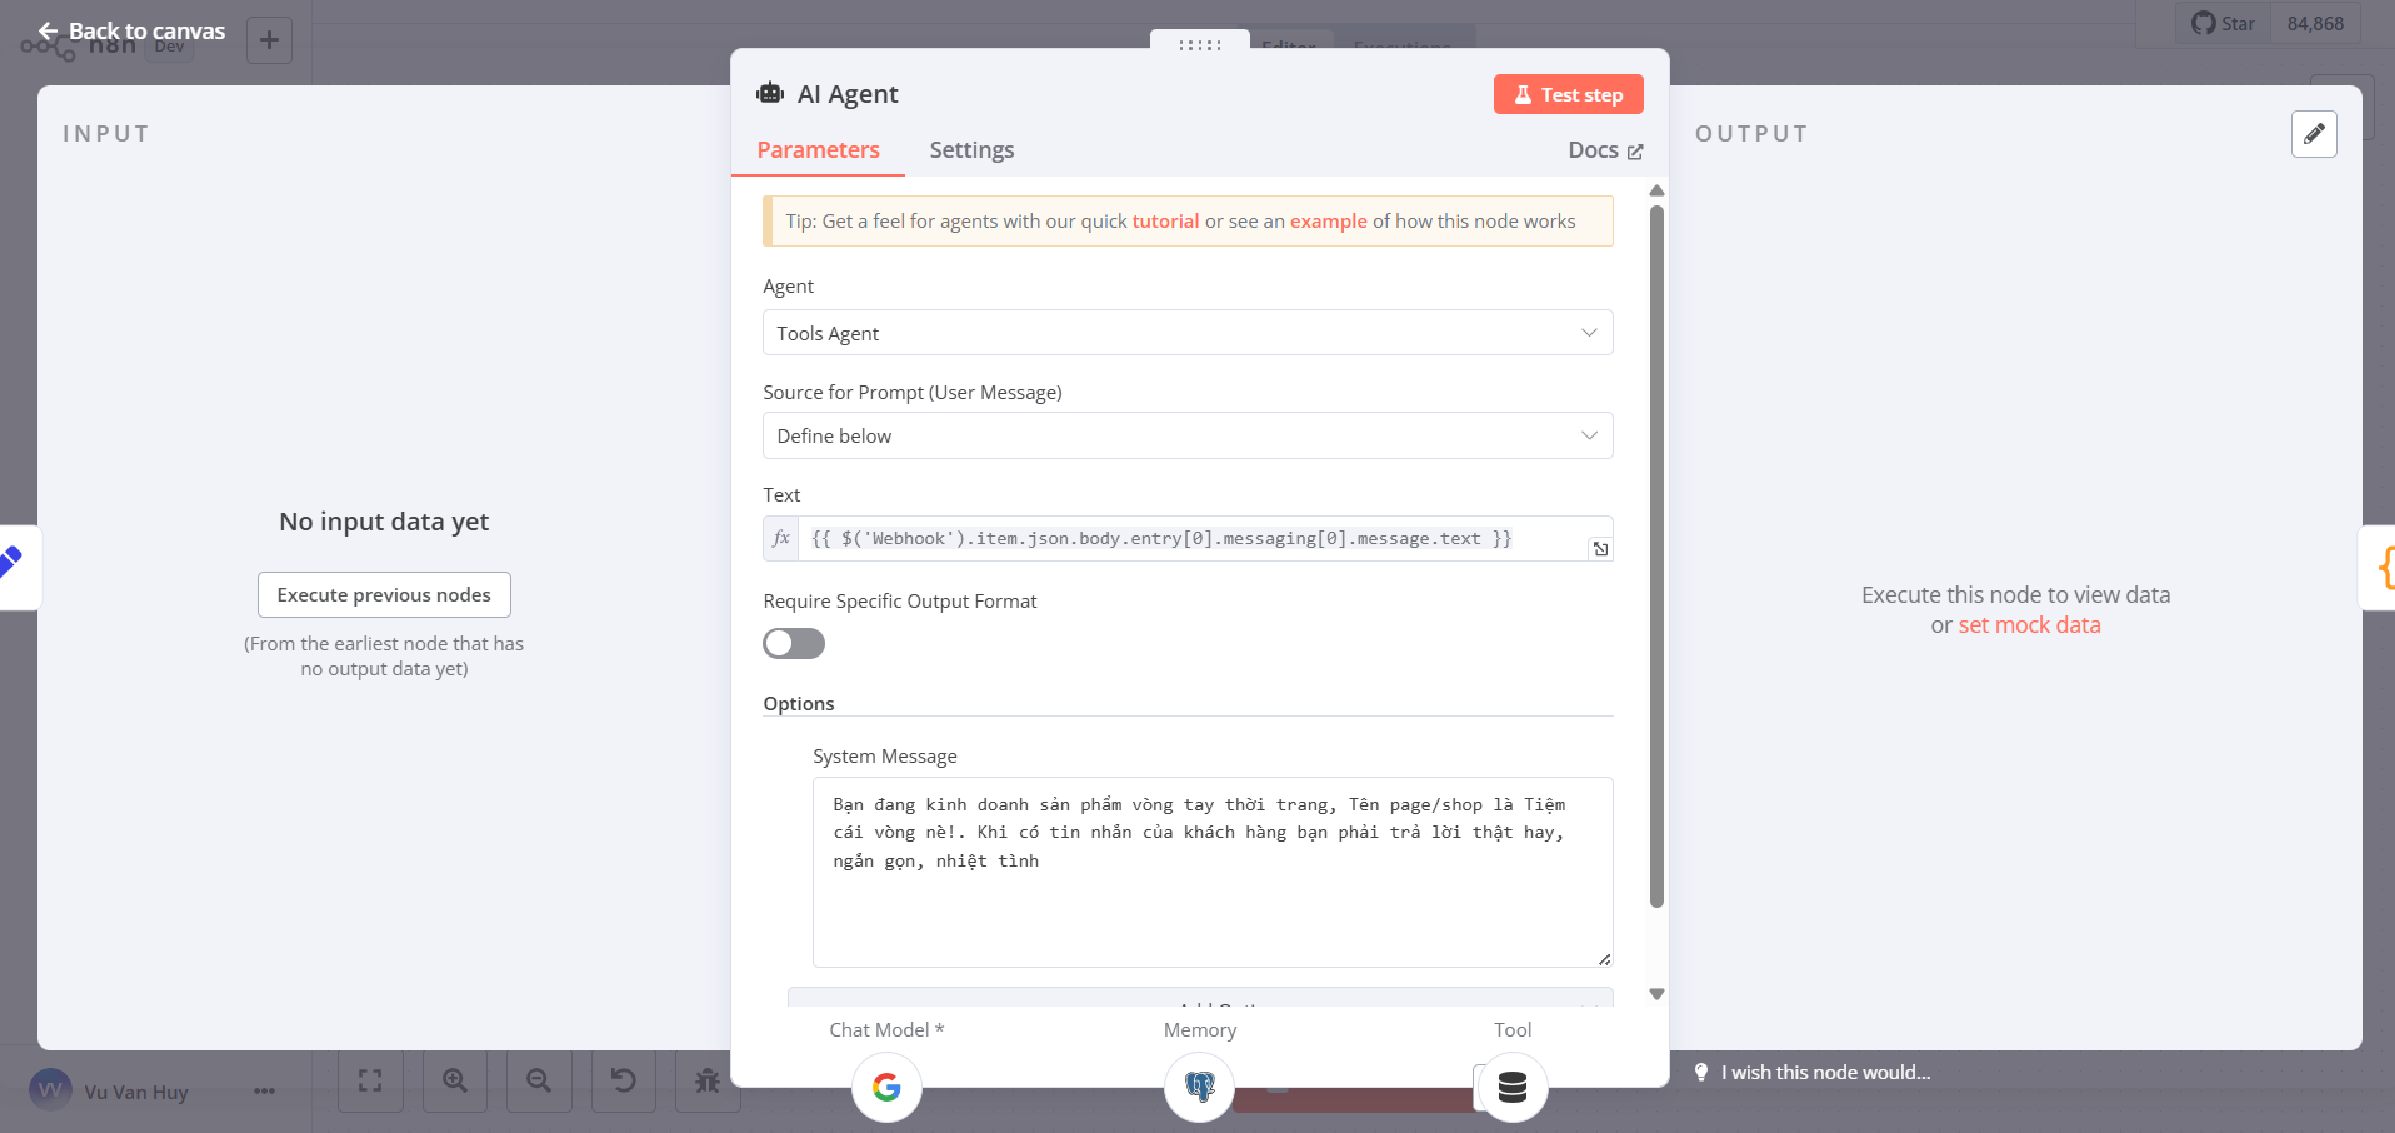
\includegraphics[width=1\linewidth]{Chap1-7/Agent-a.pdf}
\end{figure}

\begin{enumerate}
    \item Prompt – Tạo nội dung câu hỏi: 
    
    \begin{itemize}
        \item Chọn cách node nhận nội dung đầu vào (prompt) từ người dùng
        \item Tự động lấy từ node trước đó: Node sẽ lấy nội dung từ node có tên chatInput.
        \item Tự định nghĩa bên dưới: Bạn nhập văn bản tĩnh hoặc dùng biểu thức để tạo nội dung động trong phần "Prompt (User Message)".
    \end{itemize}

    \item Yêu cầu định dạng đầu ra cụ thể: Bạn có thể yêu cầu phản hồi từ AI theo định dạng nhất định chỉ bằng cách sửa prompt và yêu cầu nó. Khi bật tùy chọn này, n8n sẽ yêu cầu kết nối với một trong các node phân tích đầu ra sau:
    \begin{itemize}
        \item Auto-fixing Output Parser

        \item Item List Output Parser

        \item Structured Output Parser
    \end{itemize}

    \item Tùy chọn nâng cao cho Conversational Agent: Cho Agent biết về các công cụ  mà nó có thể thêm vào ngữ cảnh thông tin đầu vào của người dùng. Ví dụ thêm cho nó 1 cái database để select data.

\textbf{Human Message}

Đây là phần bạn mô tả:
\begin{itemize}
    \item Công cụ mà AI có thể sử dụng ({tools})

    \item Cách định dạng đầu ra ({format\_instructions})

    \item Câu hỏi hoặc yêu cầu từ người dùng ({{input}})

\end{itemize}
Một ví dụ cấu trúc thông điệp:
\begin{verbatim}
TOOLS
------
Assistant có thể yêu cầu người dùng sử dụng các công cụ sau để tìm thông tin hỗ trợ cho câu hỏi:

{tools}

{format_instructions}

USER'S INPUT
--------------------
Đây là yêu cầu của người dùng (hãy trả lời bằng đoạn mã JSON chứa một hành động duy nhất, KHÔNG thêm nội dung khác):

{{input}}
\end{verbatim}

\textbf{System Message}

Hiểu như này cho dễ hiểu. System prompt kiểu như đặt ngữ cảnh cho con chatbot hiểu. Mem có thể nhập vào đó là hãy trả lời như một ông cụ 60 tuổi chẳng hạn. Agent nó sẽ đặt mình vào bối cảnh đó và phản hồi lại cho phù hợp. Điều này làm cho con bot hiểu rõ vai trò, giọng điệu, hoặc cách phản hồi như nào sao cho đúng ý.

Ví dụ: Hãy nói chuyện như một ông cụ 60 tuổi đang khù khụ với với người bạn hiền về cuộc sống, hãy bắt đầu

Respone: À… khụ khụ… chà… lâu lắm rồi mới có người ngồi đây hàn huyên với lão già này đấy. Ờ… cái tuổi sáu mươi rồi, sáng dậy thì lưng còng, tối đến thì đầu gối kêu răng rắc… mà vẫn ham ngồi kể chuyện xưa chuyện nay. Khụ khụ…

Này… anh bạn hiền, cậu ngồi xuống đây, rót chén trà nóng đi. Thời buổi bây giờ nhanh quá… mới hôm nào còn bẻ đôi cái bánh đa, ngồi ven sông thả câu, thế mà quay đi quay lại tóc tôi đã bạc trắng thế này rồi. Anh bạn thì sao? Dạo này cuộc sống ra sao? Ừm… có cái gì vui kể lão nghe với.

$\rightarrow$ Hãy ghê :>
    \item Max Iterations: Số lần mô hình có thể chạy lặp lại để tạo ra phản hồi tốt nhất. Mặc định là 10 lần.

    \item Trả về các bước trung gian: Bạn có thể chọn bật hoặc tắt việc trả lại các bước xử lý trung gian mà agent đã thực hiện. Đây là cách hữu ích để gỡ lỗi hoặc hiểu rõ logic xử lý của mô hình AI.
\end{enumerate}


Tôi chỉ giới thiệu các option này thôi, mọi người có thể vào để nghịch nghịch thử là biết ngay à. Easy thuiii!


\subsection{OpenAI}
Node OpenAI trong n8n là cầu nối giúp bạn dễ dàng tích hợp sức mạnh của các mô hình AI hàng đầu như GPT-4, GPT-3.5, DALL·E và nhiều mô hình khác vào quy trình tự động hóa của mình. Với node này, bạn có thể thực hiện hàng loạt tác vụ thông minh như tạo văn bản, phân tích cảm xúc, tóm tắt nội dung, sinh hình ảnh và nhiều hơn thế — tất cả đều được thực hiện tự động ngay trong workflow của bạn.

OpenAI hiện là một trong những nền tảng AI phổ biến và được ứng dụng rộng rãi nhất mà n8n hỗ trợ. Nhờ node này, khả năng xử lý ngôn ngữ tự nhiên (NLP) tiên tiến của các mô hình như GPT-3 hay GPT-4 nằm gọn trong tay bạn: từ việc sinh nội dung, trả lời câu hỏi, dịch thuật, viết mã lập trình đến xây dựng chatbot hoặc trợ lý ảo.

\textbf{Bạn có thể làm được gì với OpenAI Node?}

Hãy thử tưởng tượng bạn chỉ cần nhập vài từ khóa, OpenAI sẽ tự động viết bài blog hoàn chỉnh cho bạn. Hay khi có khách hàng gửi email hỏi thông tin sản phẩm, hệ thống có thể lập tức sinh câu trả lời thông minh mà không cần ai can thiệp. Hoặc, bạn muốn tạo hình ảnh minh họa cho bài viết? Chỉ cần một prompt mô tả, DALL·E sẽ xử lý ngay.

\textbf{Cách sử dụng rất đơn giản:}

Bạn chỉ cần có API Key từ OpenAI, kết nối vào node và định nghĩa prompt — chính là câu lệnh, câu hỏi hoặc yêu cầu mà bạn muốn AI thực hiện. Ví dụ, prompt: “Hãy viết một đoạn giới thiệu ngắn về n8n bằng tiếng Việt” sẽ cho bạn kết quả trong vài giây.

Trong chương này, bạn sẽ được hướng dẫn thiết lập một workflow thực tế sử dụng OpenAI Node, để trực tiếp trải nghiệm khả năng tự động hóa kết hợp AI mạnh mẽ ngay trong n8n.



\newpage
\subsection{Basic LLM Chain}
\begin{figure}[htbp]
    \centering
    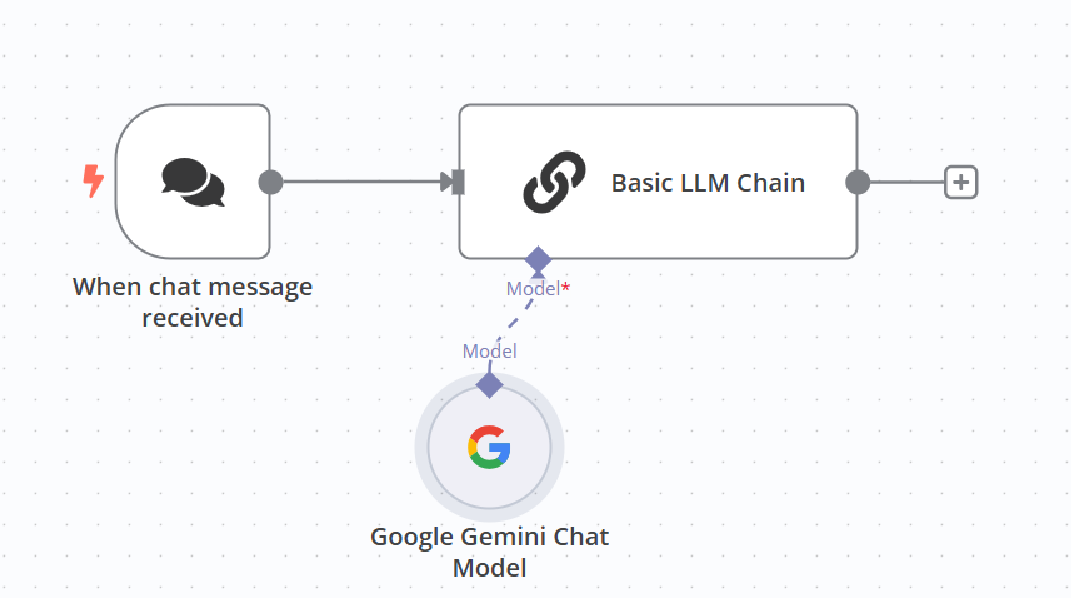
\includegraphics[width=1\linewidth]{Chap1-7/basic_llm.pdf}
\end{figure}
Basic LLM Chain là một node cơ bản nhưng cực kỳ hữu ích để làm việc với các mô hình ngôn ngữ lớn (LLM). Đây là điểm khởi đầu lý tưởng nếu bạn mới bắt đầu khám phá AI trong n8n. Node này cho phép bạn gửi một đoạn văn bản hoặc câu hỏi đến LLM và nhận lại phản hồi – đơn giản nhưng đầy tiềm năng.

Ví dụ, bạn có thể dùng Basic LLM Chain để tạo tiêu đề email tự động dựa trên nội dung, hoặc chuyển đổi một đoạn văn bản dài thành câu hỏi ngắn gọn. Cách hoạt động rất dễ hiểu: bạn cung cấp đầu vào (input), chọn mô hình LLM (như OpenAI hoặc các dịch vụ khác được hỗ trợ), và nhận đầu ra (output). Điều tuyệt vời là bạn không cần phải là chuyên gia AI để sử dụng – chỉ cần một chút sáng tạo và ý tưởng về những gì bạn muốn đạt được. Chúng ta sẽ thử một dự án nhỏ với node này để bạn làm quen ngay trong phần thực hành.
\subsection{Information Extractor}

\begin{figure}[htbp]
    \centering
    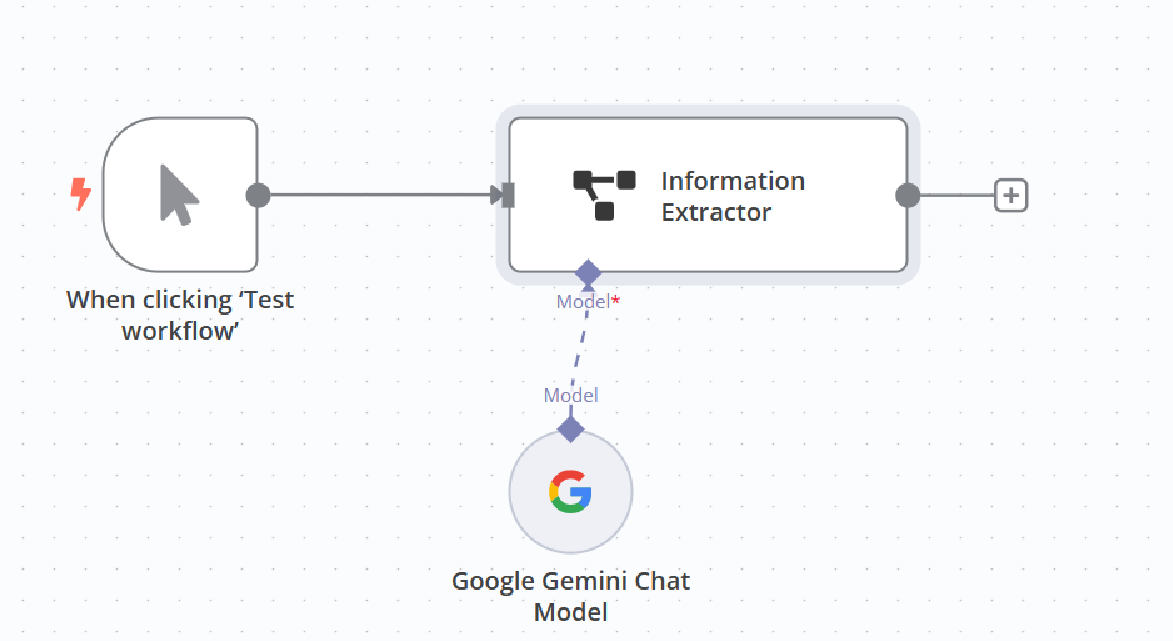
\includegraphics[width=1\linewidth]{Chap1-7/info_extract.pdf}
\end{figure}

Information Extractor là nút AI trong n8n giúp trích xuất thông tin cụ thể từ văn bản đầu vào. Nút này đặc biệt hữu ích khi bạn cần phân tích và lấy dữ liệu có cấu trúc từ nội dung phi cấu trúc như email, báo cáo, mô tả sản phẩm, bài đăng trên mạng xã hội hoặc văn bản tự do khác.

Nút này sử dụng sức mạnh của các mô hình AI để hiểu ngữ cảnh và tự động trích xuất thông tin theo cấu trúc bạn chỉ định, giúp tiết kiệm thời gian và giảm thiểu lỗi so với việc xử lý thủ công.


\textbf{Schema}

Lược đồ xác định cấu trúc của thông tin bạn muốn trích xuất. Bạn cần chỉ định một đối tượng JSON với các trường và kiểu dữ liệu tương ứng:

\begin{itemize}
    \item string: Trích xuất văn bản
    \item number: Trích xuất giá trị số
    \item boolean: Trích xuất giá trị đúng/sai
    \item array: Trích xuất danh sách các giá trị
    \item object: Trích xuất đối tượng lồng nhau với cấu trúc riêng
\end{itemize}

Hiểu đơn giản như bỏ một đoạn hồ sơ ứng viên vào sau đó nhập prompt bảo con GPT là nhặt ra cho tôi các thông tin này thông tin kia và trả về định dạng json. 

Cái này được ứng dụng nhiều trong trích xuất thông tin từ tin nhắn của khách hàng, hay email phản hồi, tự động nhập dữ liệu 



\newpage
\subsection{Question and Answer Chain}
\begin{figure}[htbp]
    \centering
    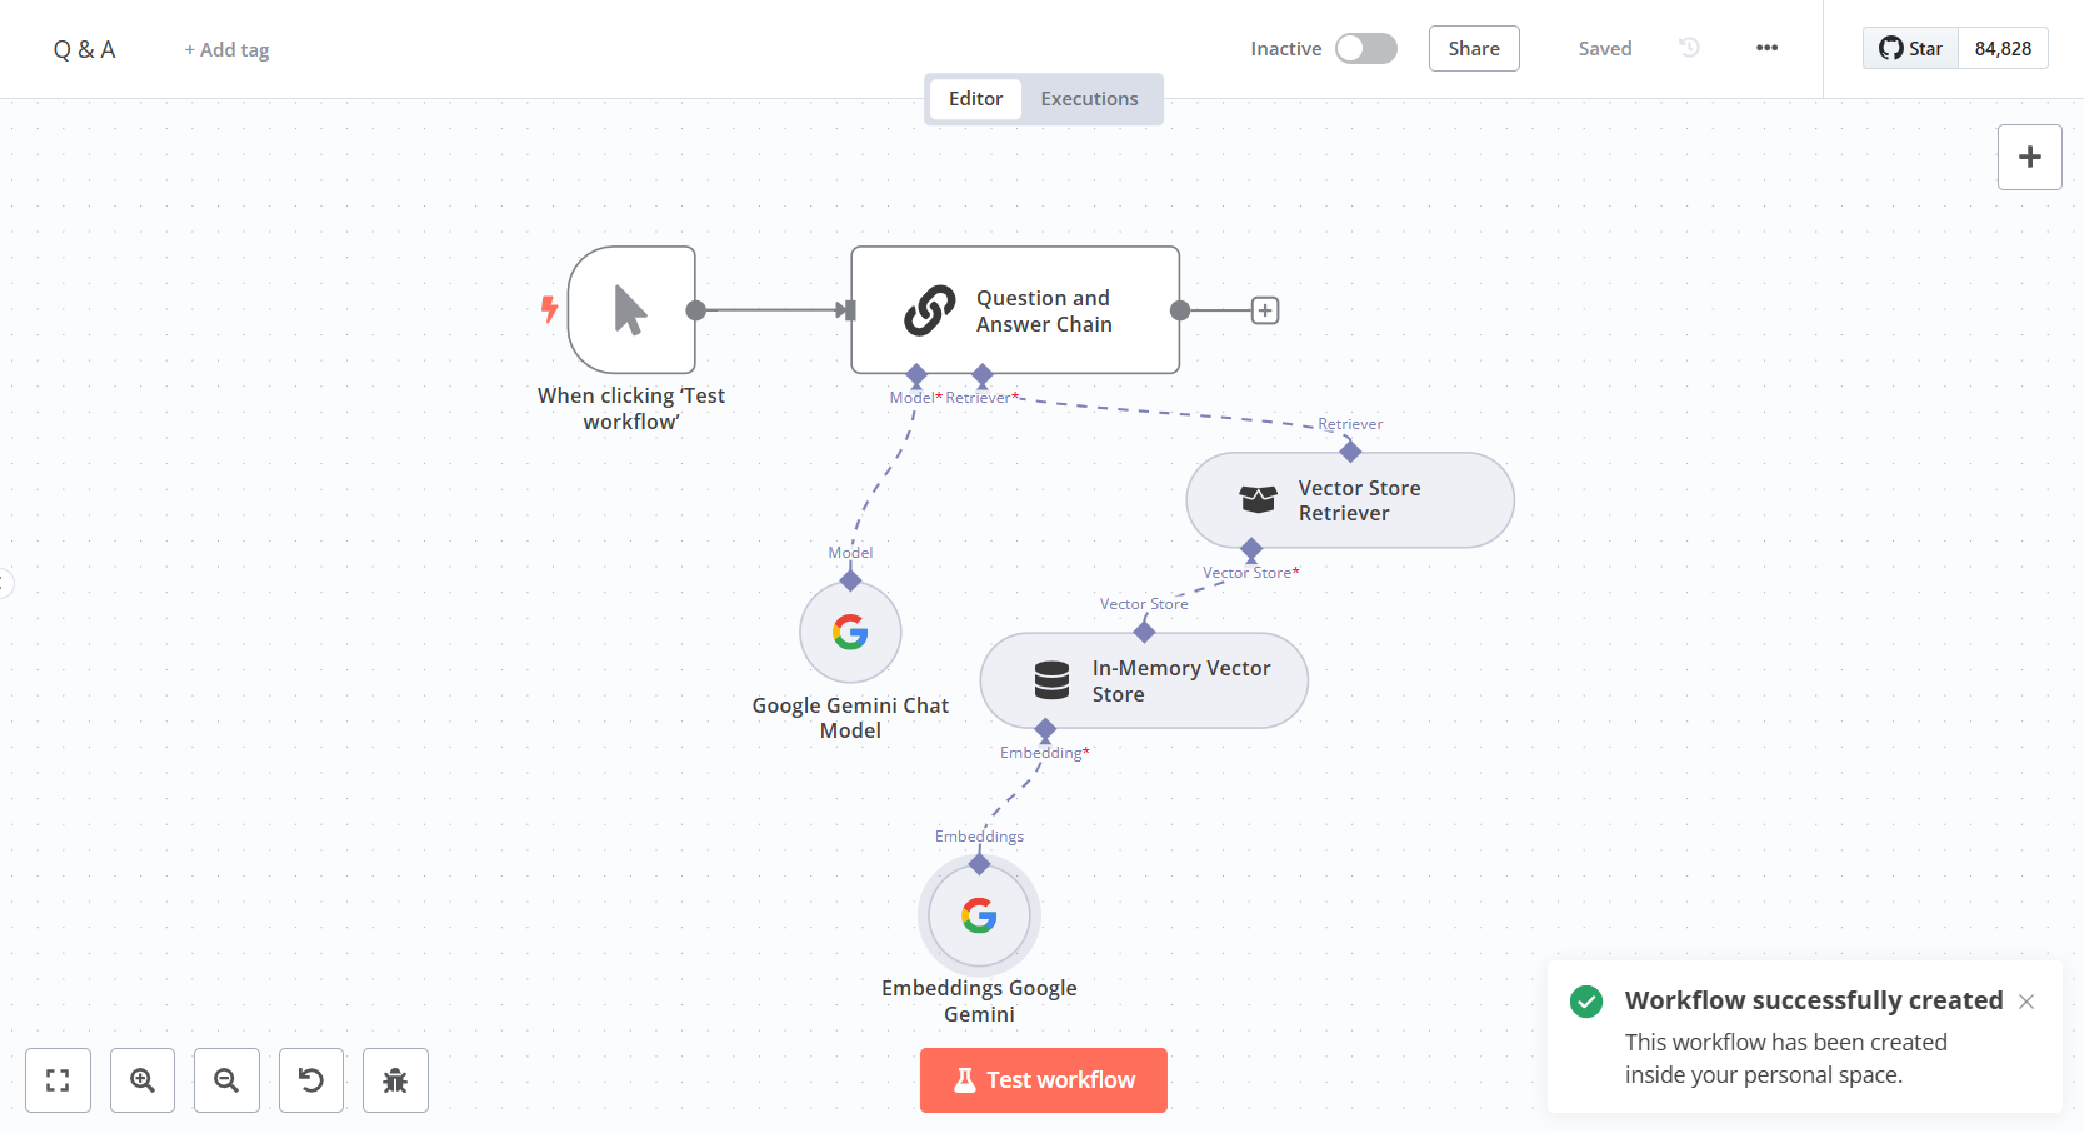
\includegraphics[width=1\linewidth]{Chap1-7/Q & A.pdf}
\end{figure}

Node này liên quan đến các bài toán liên quan đến RAG - hơi kĩ thuật hơn chút

Question and Answer Chain (Chuỗi Hỏi Đáp) là một nút AI mạnh mẽ trong n8n giúp tạo ra hệ thống trả lời câu hỏi thông minh dựa trên nguồn dữ liệu của riêng bạn. Nút này kết hợp khả năng của các mô hình ngôn ngữ lớn (LLM) với dữ liệu của bạn để tạo ra một hệ thống có thể trả lời các câu hỏi cụ thể với thông tin chính xác và phù hợp.

Điểm mạnh của Question and Answer Chain là khả năng tìm kiếm và trích xuất thông tin từ nguồn dữ liệu của bạn, sau đó sử dụng AI để tạo ra câu trả lời trôi chảy, tự nhiên dựa trên dữ liệu đó. Điều này đặc biệt hữu ích khi bạn muốn tạo ra một chatbot hoặc hệ thống trợ lý ảo có thể trả lời câu hỏi từ tài liệu nội bộ, cơ sở kiến thức hoặc nguồn dữ liệu khác.

\textbf{Cách nó hoạt động}

Question and Answer Chain hoạt động theo các bước cơ bản sau:
\begin{itemize}
    \item Nhận câu hỏi từ người dùng
    \item Tìm kiếm và truy xuất thông tin liên quan từ nguồn dữ liệu đã được cung cấp
    \item Phân tích thông tin để hiểu nội dung và ngữ cảnh
    \item Tạo câu trả lời dựa trên thông tin đã thu thập, sử dụng mô hình ngôn ngữ
    \item Trả về kết quả cho người dùng một cách tự nhiên và dễ hiểu
\end{itemize}

$\Rightarrow$ Đầu ra thường là các trợ lý ảo, chatbot thông minh.   


\subsection{Sentiment Analysis}

\begin{figure}[htbp]
    \centering
    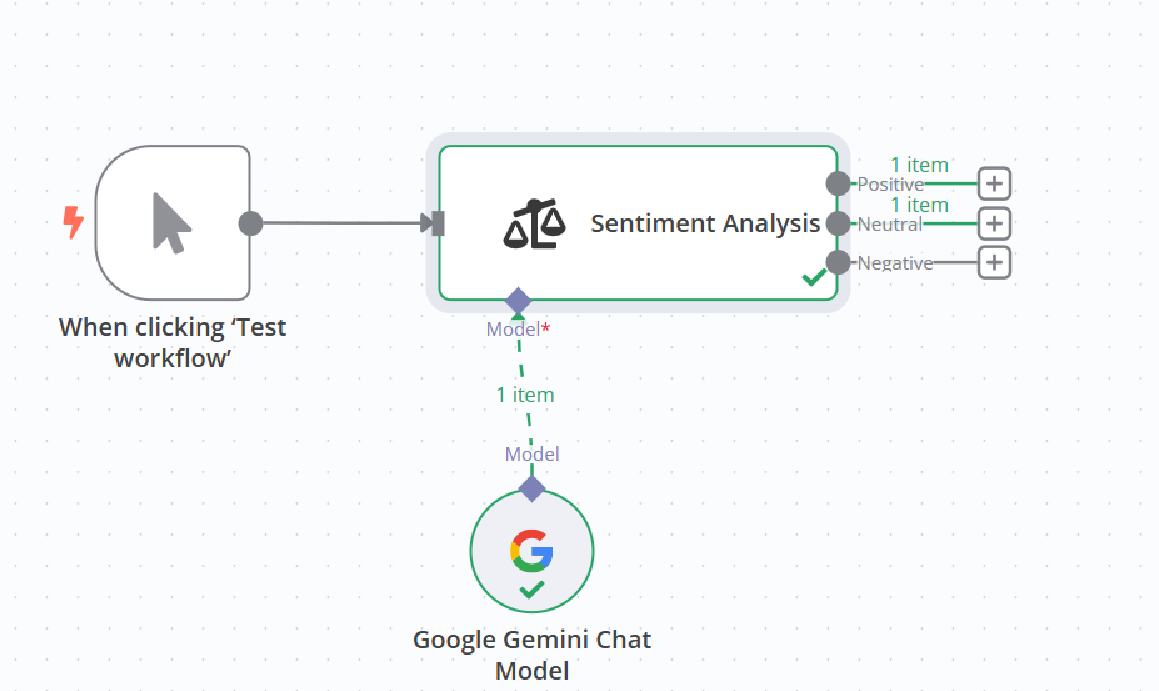
\includegraphics[width=1\linewidth]{Chap1-7/sentiment-node.pdf}
\end{figure}

Phân tích cảm xúc (Sentiment Analysis hay Opinion Mining) là một trong những ứng dụng giá trị và thiết thực nhất của AI trong lĩnh vực xử lý ngôn ngữ tự nhiên (NLP). Công nghệ này cho phép máy tính “đọc hiểu” thái độ, cảm xúc và quan điểm ẩn chứa trong văn bản — liệu chúng là tích cực, tiêu cực hay trung tính. Trong bối cảnh dữ liệu văn bản được tạo ra liên tục trên mạng xã hội, đánh giá sản phẩm, email, khảo sát… khả năng tự động phân tích cảm xúc giúp tổ chức nắm bắt phản hồi nhanh chóng, theo dõi hình ảnh thương hiệu và ra quyết định dựa trên dữ liệu thực tế.

Với n8n, bạn có thể dễ dàng xây dựng các quy trình tự động hóa để thu thập văn bản từ nhiều nguồn khác nhau, chuyển đến mô hình AI xử lý cảm xúc và thực hiện các hành động tương ứng dựa trên kết quả phân tích.

Thông thường, Sentiment Analysis sẽ phân loại văn bản vào ba nhóm chính:
\begin{itemize}
    \item Tích cực (Positive): Thể hiện sự hài lòng, khen ngợi hoặc ủng hộ.

    \item Tiêu cực (Negative): Thể hiện sự không hài lòng, phàn nàn hoặc chỉ trích.

    \item Trung tính (Neutral): Các câu thông báo, sự kiện khách quan, không chứa cảm xúc rõ ràng.
\end{itemize}


Các trường hợp ứng dụng phổ biến:
\begin{itemize}
    \item Giám sát Thương hiệu (Brand Monitoring): Tự động thu thập và phân loại cảm xúc từ các lượt đề cập thương hiệu trên mạng xã hội, diễn đàn, và báo chí — giúp doanh nghiệp kịp thời nắm bắt hình ảnh công chúng.

    \item Phân tích Phản hồi Khách hàng:
\begin{itemize}
    \item Tự động phân loại các đánh giá sản phẩm, bình luận trên trang thương mại điện tử.
    \item Đánh giá cảm xúc trong email hỗ trợ khách hàng hoặc các phiếu khảo sát mức độ hài lòng (CSAT/NPS).
\end{itemize}

    \item Quản lý Trải nghiệm Khách hàng: Xác định nhanh các khách hàng có cảm xúc tiêu cực để ưu tiên hỗ trợ, chăm sóc hoặc xử lý sự cố.

    \item Nghiên cứu Thị trường: Phân tích cảm xúc cộng đồng đối với sản phẩm mới, chiến dịch quảng cáo hoặc các xu hướng xã hội.

    \item Phân loại Nội dung: Tự động gắn nhãn cảm xúc cho bài viết, bình luận trên diễn đàn, mạng xã hội hay website.

\end{itemize}


\subsection{Summarization Chain}
Trong kỷ nguyên bùng nổ thông tin như hiện nay, nhu cầu tóm tắt văn bản ngày càng trở nên thiết yếu. Từ email, báo cáo, bài báo cho đến bản ghi cuộc họp, việc nhanh chóng nắm bắt nội dung chính giúp tiết kiệm thời gian và nâng cao hiệu quả làm việc.

Sự phát triển vượt bậc của Trí tuệ nhân tạo, đặc biệt là các Mô hình Ngôn ngữ Lớn (LLMs), đã mở ra khả năng tóm tắt văn bản một cách tự nhiên và chính xác. Không chỉ dừng lại ở việc phân tích dữ liệu thô, AI giờ đây có thể tạo ra những bản tóm tắt súc tích, đúng trọng tâm và phù hợp với ngữ cảnh sử dụng.

Trong bối cảnh đó, n8n nổi lên như một nền tảng tự động hóa linh hoạt, cho phép người dùng xây dựng các quy trình xử lý dữ liệu kết hợp với sức mạnh của AI. Đặc biệt, với tính năng thiết lập các chuỗi workflow (chains), n8n giúp kết nối nhiều bước xử lý khác nhau — từ tiếp nhận văn bản, truyền dữ liệu đến AI, lấy kết quả tóm tắt và gửi đi hoặc lưu trữ. Summarization Chain chính là một workflow như vậy, được thiết kế chuyên biệt để tự động hóa việc tóm tắt nội dung.

Các trường hợp ứng dụng phổ biến:

\begin{itemize}
    \item Tóm tắt Email/Chuỗi Email: Tự động trích xuất và tổng hợp ý chính từ các email quan trọng hoặc các cuộc trao đổi dài dòng.

    \item Tóm tắt Báo cáo/Tài liệu: Rút gọn nội dung của báo cáo doanh nghiệp, tài liệu kỹ thuật hoặc nghiên cứu chuyên sâu, giúp người đọc nắm được thông tin trọng yếu nhanh chóng.

    \item Tóm tắt Bản ghi Cuộc họp: Chuyển bản ghi họp thành danh sách các quyết định và nhiệm vụ hành động ngắn gọn, dễ theo dõi.

    \item Tóm tắt Tin tức/Bài báo: Tạo feed tin tức cá nhân hóa với bản tóm tắt ngắn gọn từ nhiều nguồn báo chí khác nhau.

    \item Phân tích Phản hồi Khách hàng: Tổng hợp những ý kiến nổi bật từ hàng trăm đánh giá, khảo sát hoặc bình luận mạng xã hội.

    \item Tạo Mô tả ngắn (Abstracts): Tự động sinh bản tóm tắt cho bài viết blog, báo cáo khoa học hoặc nội dung truyền thông.
\end{itemize}

Lựa chọn Mô hình AI và Tinh chỉnh (Choosing Models \& Fine-tuning):
\begin{itemize}
    \item GPT-4/Claude 3 Opus: Chất lượng cao nhất, hiểu ngữ cảnh tốt, nhưng đắt hơn và chậm hơn.
    \item GPT-3.5 Turbo/Claude 3 Sonnet/Gemini Pro: Cân bằng tốt giữa chi phí, tốc độ và chất lượng. Thường là lựa chọn tốt để bắt đầu.
    \item Hugging Face/Ollama: Linh hoạt, có thể chọn mô hình chuyên biệt cho tóm tắt, có thể chạy cục bộ (Ollama) để tiết kiệm chi phí hoặc bảo mật dữ liệu, nhưng đòi hỏi cấu hình phức tạp hơn.
    \item Prompt Engineering: Nhấn mạnh tầm quan trọng của việc viết prompt rõ ràng, chi tiết. Thử nghiệm với các kiểu prompt khác nhau để đạt kết quả tốt nhất (ví dụ: yêu cầu độ dài cụ thể, giọng văn, đối tượng người đọc, các điểm cần tập trung).
    \item Tham số Model: Giới thiệu sơ qua về các tham số như temperature (ảnh hưởng độ sáng tạo/ngẫu nhiên), max\_tokens (giới hạn độ dài output).
\end{itemize}


\section{Khi Tự Động Hóa Gặp Trí Tuệ Nhân Tạo}
Tôi vẫn nhớ dự án đầu tiên suýt "đổ bể" khi cố gắng tích hợp AI vào quy trình kinh doanh. Hồi đó, tôi nghĩ việc kết nối các dịch vụ AI sẽ đơn giản như việc nối các đoạn ống nước. Thực tế hoàn toàn khác.


\subsection{Dự Án Điển Hình 1: Hệ Thống Quản Lý Khiếu Nại Thông Minh}
\textbf{Bối Cảnh Thực Tế:}

Một công ty logistics tiếp nhận hơn 500 khiếu nại mỗi tháng qua email, điện thoại và mạng xã hội. Nhân viên phải xử lý thủ công bằng giấy tờ và file Excel, gây quá tải và dễ sai sót. Hệ thống cũ không thể theo dõi, tổng hợp hay cảnh báo kịp thời, ảnh hưởng đến trải nghiệm khách hàng và uy tín công ty.

Giải pháp bằng AI: sử dụng n8n để tự động thu thập khiếu nại từ email, form và API mạng xã hội, lưu vào cơ sở dữ liệu tập trung. Kết hợp AI để phân loại nội dung khiếu nại theo mức độ ưu tiên và chủ đề. Hệ thống sẽ tự động gửi thông báo đến bộ phận liên quan và cập nhật trạng thái xử lý. Ngoài ra, n8n còn tạo báo cáo hàng ngày và gửi email thống kê cho quản lý mà không cần thao tác thủ công.



\subsection{Dự án Điển Hình 2: Trích xuất thông tin từ kho dữ liệu hồ sơ ứng viên}


% Bạn là một HR, hằng ngày bạn phải mày mò phát nhọc với hàng loạt CV của ứng viên. Đối với các ngân hàng lớn, big tech như viettel, cmc. Mỗi đợt tuyển dụng sẽ có lượng hồ sơ kinh khủng. Để sử lý lượng CV này đòi hỏi nhiều thời gian và công sức

Tuyển dụng là một quá trình tốn nhiều thời gian và nguồn lực, thường đầy rẫy thách thức. Từ việc tìm kiếm và sàng lọc ứng viên đến tiến hành phỏng vấn và đánh giá nhân tài, các nhà tuyển dụng cần phải điều hướng nhiều nhiệm vụ khác nhau để tìm ra ứng viên phù hợp với nhu cầu của công ty. Theo nghiên cứu của Glassdoor - Website tổng hợp đánh giá của nhân viên về doanh nghiệp họ đã và đang làm việc, trung bình doanh nghiệp mất 23 ngày để tìm kiếm ứng viên phù hợp và 1/3 thời gian trong tháng sử dụng để phỏng vấn ứng viên. Nhưng với sự phát triển của AI, nhiều nhiệm vụ trong số này hiện có thể được đơn giản hóa và tự động hóa, giúp các nhà quản lý tuyển dụng tiết kiệm thời gian và nguồn lực. Workflow này ra đời nhằm giải quyết vấn đề này, hỗ trợ người HR giảm thiểu thời gian tìm kiếm ứng viên phù hợp thông qua việc tương tác với chatbot, được huấn luyện bởi các mô hình ngôn ngữ lớn, và áp dụng các kỹ thuật tối ưu cho bài toán tìm kiếm thông tin.













Bằng cách sử dụng giải pháp này, các nhà tuyển dụng có thể tiết kiệm thời gian và công sức, cải thiện chất lượng ứng viên phù hợp, giảm thiên vị và đưa ra quyết định dựa trên dữ liệu. AI cho tuyển dụng có tiềm năng cách mạng hóa bối cảnh tuyển dụng bằng cách tăng hiệu quả, độ chính xác và hiệu quả chung trong việc xác định và thu hút nhân tài phù hợp cho các tổ chức. Trong khi các nhà tuyển dụng có thể dành vô số giờ để thẩm định nhân viên tiềm năng, phần mềm AI có thể xử lý lượng dữ liệu khổng lồ và chỉ trong vài giờ hoặc thậm chí vài phút, phân tích những ứng viên tiềm năng nào có thể phù hợp với công việc. Phần mềm AI có thể khớp trình độ và yêu cầu công việc với kỹ năng và kinh nghiệm của ứng viên, nhanh chóng phân loại sơ yếu lý lịch không phù hợp. Bộ phận nhân sự cũng có thể làm cho quy trình tuyển dụng hiệu quả hơn và tiết kiệm thời gian, cuối cùng giúp các nhà tuyển dụng tiết kiệm tiền. Đây là khía cạnh quan trọng cần cân nhắc khi nói đến tài chính của bất kỳ doanh nghiệp nào. Việc hợp lý hóa quy trình tuyển dụng, tuyển dụng và tuyển dụng sẽ giúp giảm chi phí, dẫn đến sự kết hợp thuận lợi giữa chi phí thấp hơn và năng suất tăng lên.